\documentclass[10pt]{article}
\usepackage[
  top    = 0.5in,
  left   = 0.5in,
  right  = 2.5in,
  %bottom = 4.5in,
  %showframe
]{geometry}
\usepackage{pgfplots}
\usetikzlibrary{patterns,calc}
\pgfplotsset{
  compat=1.18,
}
\tikzset{
  myaxis/.append style={
    ->,
    ultra thick
  },
  mygrid/.append style={
    dotted, thick
  },
  myminorgrid/.append style={
    dotted, thin
  },
  ball/.append style={
    shading=ball,
    minimum width=15pt
  },
  ground/.append style={
    pattern=north east lines
  },
  vel/.append style={
    ->,
    ultra thick,
    red
  },
  vellab/.append style={
    right=2pt,
  },
}

\begin{document}
\pagestyle{empty}

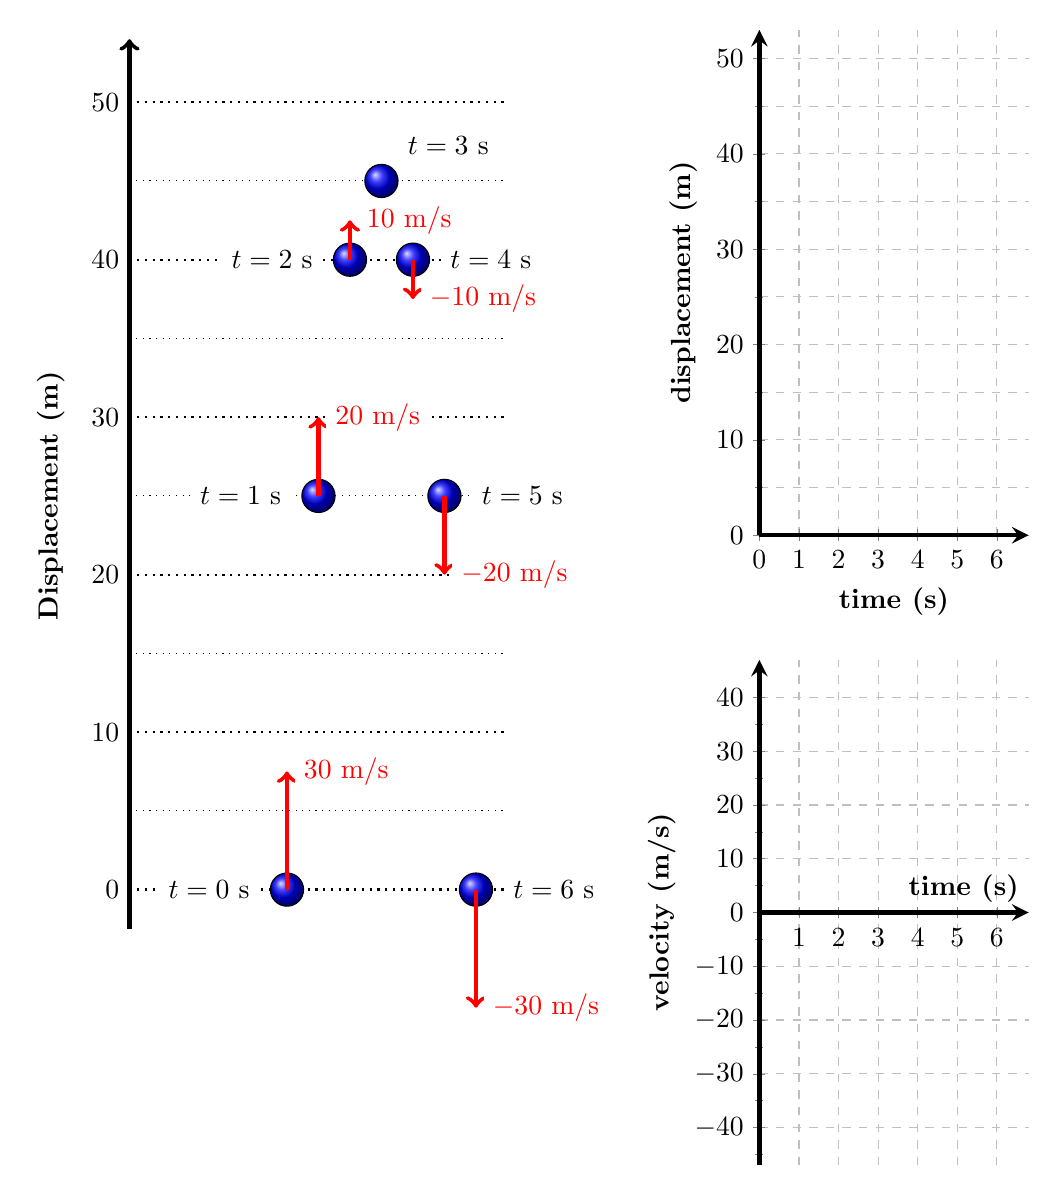
\begin{tikzpicture}
  \begin{scope}[every node/.append style={fill=white}]
    \def\scale{0.2}
    \def\xscale{0.4}
    \def\axisloc{-2}
    \def\velscale{.05}
    \draw[myaxis] (\axisloc,-.5) -- (\axisloc,54*\scale);
    \node[rotate=90] at (-3,25*\scale) {\bf Displacement (m)};
    \foreach \y in {0,10,20,...,50} {
      \draw[mygrid] (\axisloc,\scale*\y) node[anchor=east,fill=none] {\y} -- (\xscale*7,\scale*\y);
    }
    \foreach \y in {5,15,...,50} {
      \draw[myminorgrid] (\axisloc,\scale*\y) -- (\xscale*7,\scale*\y);
    }
    %\fill[ground] (\axisloc,0) rectangle (7*\xscale,-0.5);

    \draw[ball] (0,0) coordinate (a) 
      circle (6pt)
      node[left=10pt] {$t=0$ s};
    \draw[ball] (\xscale*1,\scale*25) coordinate (b) 
      circle (6pt) 
      node[left=10pt] {$t=1$ s};
    \draw[ball] (\xscale*2,\scale*40) coordinate (c)
      circle (6pt) 
      node[left=10pt] {$t=2$ s};
    \draw[ball] (\xscale*3,\scale*45)  coordinate (d)
      circle (6pt)
      node[above right=6pt] {$t=3$ s};
    \draw[ball] (\xscale*4,\scale*40) coordinate (e)
      circle (6pt)
      node[right=10pt] {$t=4$ s};
    \draw[ball] (\xscale*5,\scale*25) coordinate (f) 
      circle (6pt) 
      node[right=10pt] {$t=5$ s};
    \draw[ball] (\xscale*6,0) coordinate (g)
      circle (6pt)
      node[right=10pt] {$t=6$ s};

    \draw[vel] (a) -- ++ (0,30*\velscale) 
      node[vellab] {$30$ m/s};
    \draw[vel] (b) -- ++ (0,20*\velscale) 
      node[vellab] {$20$ m/s};
    \draw[vel] (c) -- ++ (0,10*\velscale) 
      node[vellab,fill=none] {$10$ m/s};
    \draw[vel] (e) -- ++ (0,-10*\velscale) 
      node[vellab] {$-10$ m/s};
    \draw[vel] (f) -- ++ (0,-20*\velscale) 
      node[vellab] {$-20$ m/s};
    \draw[vel] (g) -- ++ (0,-30*\velscale) 
      node[vellab] {$-30$ m/s};
  \end{scope}
  
  \begin{scope}[shift={(6,4.5)}]
    \begin{axis}[
      axis y line = left,
      axis x line = bottom,
      axis line style = ultra thick,
      xlabel={\bf time (s)},
      ylabel={\bf displacement (m)},
      ymin=0,
      ymax=53,
      xmin=0,
      xmax=6.8,
      ytick={-10,0,10,...,50},
      xtick={0,...,7},
      minor y tick num = 1,
      grid style = {dashed},
      grid=both,
      width=5cm,
      height=8cm,
    ]
    \end{axis}
  \end{scope}

  \begin{scope}[shift={(6,-3.5)}]
    \begin{axis}[
      xlabel={\bf time (s)},
      ylabel={\bf velocity (m/s)},
      ymin=-47,
      ymax=47,
      xmin=0,
      xmax=6.8,
      ytick={-50,-40,...,50},
      xtick={0,...,7},
      minor y tick num = 1,
      grid style = {dashed},
      grid=major,
      axis y line = left,
      axis x line = center,
      axis line style = ultra thick,
      width=5cm,
      height=8cm,
    ]
    \end{axis}
  \end{scope}

\end{tikzpicture}

\vspace{\stretch{1}}
cut 2 inches off right; cut 4 inches off bottom



\end{document}